\documentclass[12pt,a4paper]{article}
\usepackage{amsmath}
\usepackage{amsfonts}
\usepackage{graphicx}
\usepackage{relsize}
\usepackage{listings,lstautogobble}
\usepackage{xcolor}
\usepackage[numbered, framed]{matlab-prettifier}
\usepackage[margin=0.6in]{geometry}

\graphicspath{ {.} }
\newcommand{\bint}{\mathop{\mathlarger{\int}}}
\lstset{keywordstyle=\color{magenta},
        style=Matlab-editor,
        language=matlab, 
        basicstyle=\small,
        autogobble=true}

\begin{document}
    \Large{\textbf{Q4.1:}}

    \textbf{(a)} $$\int_{-\infty}^\infty dt\ y(t)(\frac{d}{dt}step(t-t_0))
    =\int_{-\infty}^\infty dt\ y(t) \delta(t-t_0)
    =y(t_0)$$

    \textbf{(b)} $$\int_0^\infty dt\ y(t)-\int_{-\infty}^{0}dt\ y(t) = \int_0^\infty dt\ 1*y(t) + \int_{-\infty}^{0} dt\ (-1)*y(t)$$
    
    To make $\bint_{-\infty}^\infty dt\ y(t)\psi(t)$ equal previous term, 
    $\psi(t)=
    \begin{cases}
    1  & t \ge 0 \\
    -1 & t < 0
    \end{cases}$

    \newpage
    \Large{\textbf{Q4.2:}}

    \noindent \textbf{(a).}
    $\psi_{gg}(t)=\bint_{-\infty}^\infty dt'\ g(t')g(t'-t)
    =\bint_{-\infty}^\infty dt'\ e^{-\frac{t'^2}{2\sigma^2}} * e^{-\frac{(t'-t)^2}{2\sigma^2}} \\
    =\bint_{-\infty}^\infty dt'\ e^{-\frac{1}{\sigma^2}t'^2+\frac{t}{\sigma^2}t'} * e^{-\frac{t^2}{2\sigma^2}}
    =e^{-\frac{t^2}{2\sigma^2}} \bint_{-\infty}^\infty dt'\ e^{-\frac{1}{\sigma^2}t'^2+\frac{t}{\sigma^2}t'}$\\
    So $a=\frac{1}{\sigma}, b=\frac{t}{\sigma^2}$, then \\
    $\psi_{gg}(t)=e^{-\frac{t^2}{2\sigma^2}}*\sqrt{\pi\sigma^2}e^{\frac{t^2}{4\sigma^2}}=\sigma\sqrt{\pi}e^{-\frac{t^2}{4\sigma^2}}$

    \noindent \textbf{(b).} Let $t-\tau=\tau_0$, then $t=\tau+\tau_0$ and $\tau=t-\tau_0$
    \begin{figure}[!ht]
        \centering
        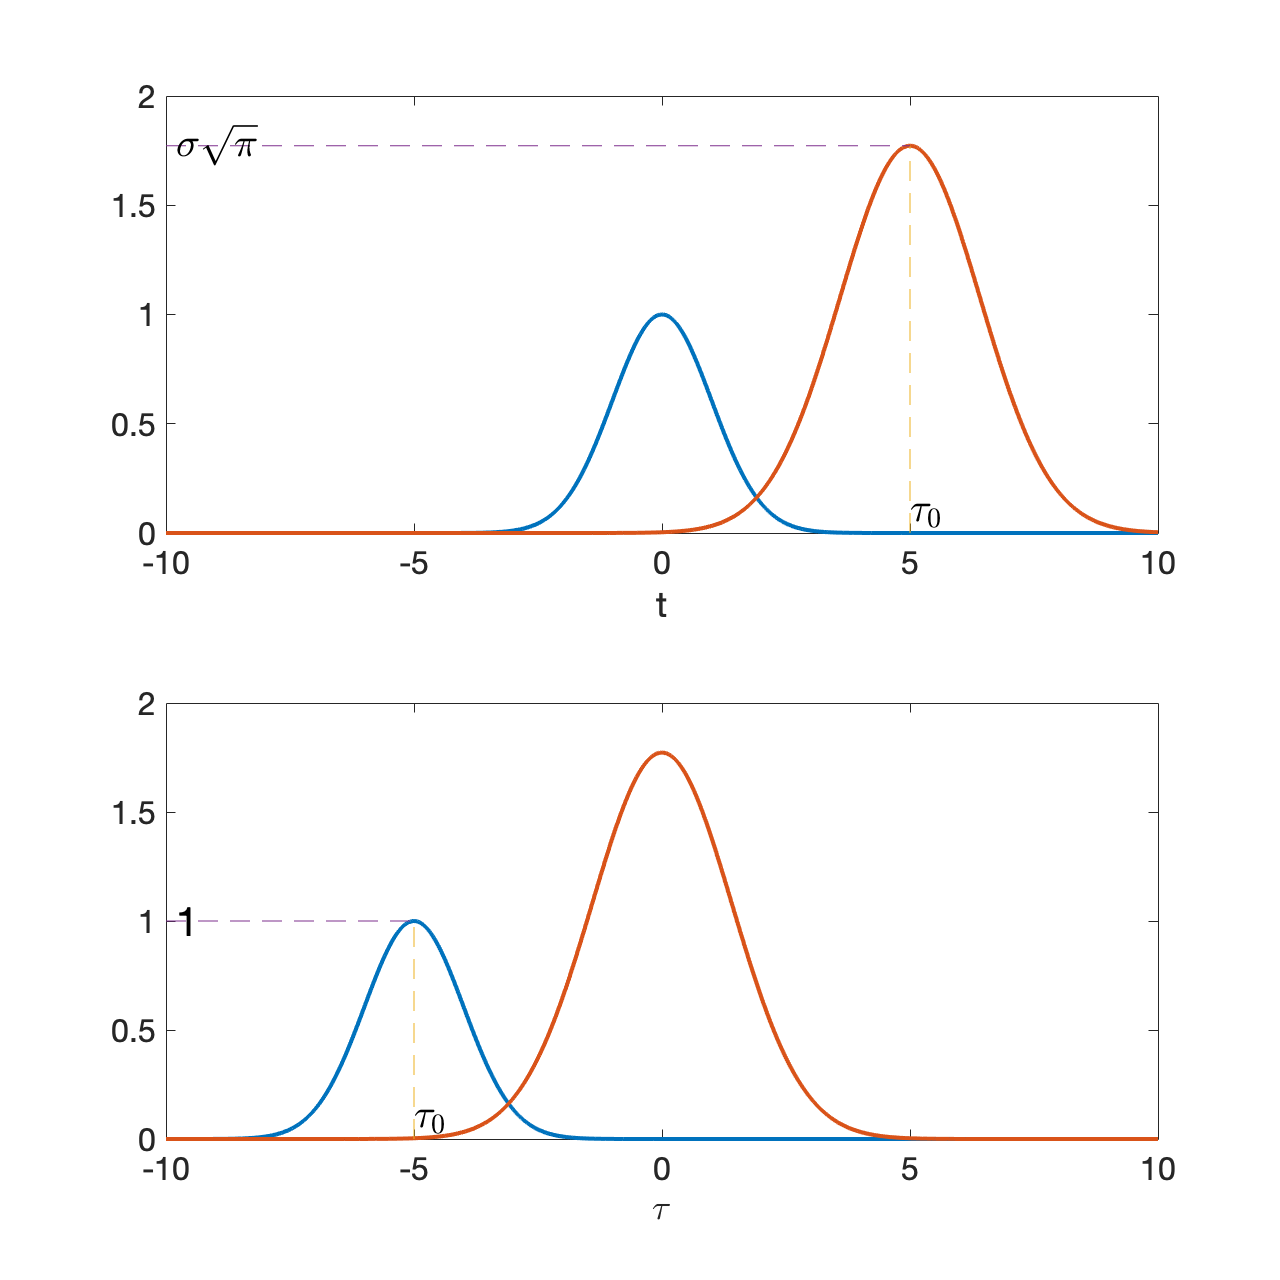
\includegraphics[width=0.8\textwidth]{g_psi.png}
        \vspace{-0.5cm}
        \label{fig:1}
        \caption{The upper image is puting $\psi(\tau)$ onto $g(t)$ and the lower one is $g(t)$ on $\psi(\tau)$ }
    \end{figure}

    \noindent \textbf{(c).}
    For $g(t)=e^{-\frac{t^2}{2\sigma^2}}$, it has maximumm value at $t=0$: $max\ g(t) = g(0)=1$. So its FWHM value is the solution of $e^{-\frac{t^2}{2\sigma^2}}=1/2 \longrightarrow t_{FWHM}=\sigma\sqrt{2ln2}$.

    \noindent For $\psi(\tau)=\sqrt{\pi\sigma^2}e^{-\frac{t^2}{4\sigma^2}}$, $t_{FWHM}=2\sigma\sqrt{ln2}$

    \noindent So their ratio is: $\frac{\sigma\sqrt{2ln2}}{2\sigma\sqrt{ln2}}=\frac{1}{\sqrt{2}}$

    \newpage
    \Large{\textbf{Q4.4}}
    
    \textbf{(a).} $SNR=\frac{var(s(t))}{var(e(t))}-1=\frac{var(gg)}{var(nois)}=0.144$

    \textbf{(b).}
    \begin{enumerate}
        \item Suppress noise with gaussian matched filter \\
        design 2D gaussian filter as $K(x, y)=exp(\frac{-x^2}{2\sigma^2})\ for\ y \le L/2$ where $L$ is the filter kernel size. Then rotate the kernel to get rotated filter with every 30 degree, in order to fit cell walls oriented at any angle. Then use $conv$ to apply the all the filters to the raw image with noise and retain the maximum activation signal. By setting the $\sigma=1,L=9$, the $SNR$ increases to $13.0478$.
        \begin{figure}[!ht]
            \centering
            \includegraphics*[width=\textwidth]{g_fil.png}
            \label{fig:2}
            \caption{Raw image with noise VS image after applying gaussian filter}
        \end{figure}
        
        \vspace{-0.5cm}
        Code: \\
        \vspace{-0.5cm}
        \begin{lstlisting}
        out=zeros(size(gg));
        s=1;L=9;
        m=(L-1)/2;
        [x,y]=meshgrid(-m:m,-m:m); 
        % from 0 to 150 with 30 as interval
        theta=0:30:150;  
        for t=theta
            % rotate 
            u = cos(t)*x - sin(t)*y; 
            v = sin(t)*x + cos(t)*y;
            N = (abs(u)<=m) & (abs(v)<=m);
            k = exp(-u.^2/(2*s.^2)); % filter
            k = k - mean(k(N));
            k(~N) = 0;
            res = conv2(gg, k, 'same');
            out = max(out, res);
        end
        \end{lstlisting}

        \item Detect cells with circle filter\\
        Because the shape of cells is circle or ellipse, so we could design circle filter by: 
        \lstinline[language=matlab]{fspecial('disk', r)}, where \textbf{r} is the radius of the circle filter. Like what we did in step, we range \textbf{r} from 3 to 12 and iteratively apply the obtained circle filter to denoised image via gaussian filter, then keep the maximum activation outputs. Clustering the locations with maximum activation value should be consistent with the cell locations. 
    \end{enumerate}

    \newpage
    \Large{\textbf{Q4.5}}

    $g(t)=[h*f](t)=\bint_{-\infty}^\infty dt'h(t-t')f(t')\\
    \indent =\bint_{-\infty}^\infty dt' \frac{1}{\tau}exp(\frac{t'-t}{\tau})step(t-t') rect(\frac{t'}{2T_0})$

    where $step(t-t')=\begin{cases}
    1; & t'\le t\\
    0; & t'>0
    \end{cases}$,  
    and $rect(\frac{t'}{2T_0})=\begin{cases}
    1; & -T_0 \le t' \le T_0 \\
    0; & t' > T_0\ or\ t' < -T_0
    \end{cases}$

    Therefore, $g(t)$ has 3 cases due to the relationship between $t$ and $T_0$:
    \begin{enumerate}
    \item when $t\ge T_0$, the rect is entirely covered by $step=1$ area, so \\
    $g(t)=\bint_{-T_0}^{T_0}dt' \frac{1}{\tau}exp(\frac{t'-t}{\tau})=exp(\frac{t'-t}{\tau})\bigg|_{-T_0}^{T_0}=exp(\frac{T_0-t}{\tau})-exp(\frac{-T_0-t}{\tau})$
    \item when $-T_0\le t<T_0$, the rect is partially covered by $step=1$ area, so \\
    $g(t)=\bint_{-T_0}^{t}dt' \frac{1}{\tau}exp(\frac{t'-t}{\tau})=exp(\frac{t'-t}{\tau})\bigg|_{-T_0}^{t}=1-exp(\frac{-T_0-t}{\tau})$
    \item when $t < -T_0$, the rect has no overlap with $step=1$ area, which means their multiplication value is all 0. \\
    $g(t)=0$
    \end{enumerate}

    \newpage
    \Large{\textbf{Q4.6}}
    
    Let $\mathbf{H}=\frac{100}{m}rect(\frac{t-0.01m}{0.02m})$, where $m=1,2,...,1000$. 
    \begin{figure}[!ht]
        \centering
        \includegraphics*[width=0.9\textwidth]{ltv.png}
        \label{fig:3}
        \caption{$g(t)$ when applying LTV response $\mathbf{H}$ to $f[n]$}
    \end{figure}

    Code: \\
    \vspace{-0.5cm}
    \begin{lstlisting}[basicstyle=\large]
    t=0:0.01:9.99;
    fn=cos(2*pi.*t);
    N = length(t);
    h1 = zeros(N, 1);
    h1(1) = 100;
    H(1, :) = h1;
    for j=2:N
        h = zeros(N, 1);
        h(1:j) = 1/(j*0.01);
        H(j, :) = h;
    end
    g = H*fn';
    \end{lstlisting}


\end{document}